\documentclass[12pt]{article}
\usepackage[a4paper, margin=.30in]{geometry}
%\usepackage{array}
\usepackage{graphicx, subfig, wrapfig, makecell,fancybox }
 \usepackage[version=4]{mhchem}
\newcommand\headerMe[2]{\noindent{}#1\hfill#2}
\renewcommand \thesection{\Roman{section}}

\newcolumntype{M}[1]{>{\raggedright}m{#1}}



\begin{document}

\headerMe{Royaume du Maroc}{année scolaire \emph{2021-2022}}\\
\headerMe{Ministère de l'Éducation nationale, }{  Professeur :\emph{Zakaria Haouzan}}\\
\headerMe{du Préscolaire et des Sports}{Établissement : \emph{Lycée SKHOR qualifiant}}\\

\begin{center}
Devoir surveillé N°2 \\
1Bac Sciences Expérimentales\\
Durée 2h00
\\
    \vspace{.2cm}
\hrulefill
\Large{Fiche Pédagogique}
\hrulefill\\
\end{center}
%end Headerss------------------------


%__________________Chimie ______________________-
%%%%%%%+_+_+_+_+_+_+_+_+_Partie1
\section[A]{Introduction }
\hspace{0.5cm}Le programme d'études de la matière physique chimie vise à croître un ensemble de compétences visant à développer la personnalité de l'apprenant. Ces compétences peuvent être classées en Compétences transversales communes et Compétences qualitatives associées aux différentes parties du programme.
\section{cadre de référence }
 \hspace{0.5cm}L'épreuve a été réalisée en adoptant des modes proches à des situations d'apprentissages et des situations problèmes, qui permettent de compléter les connaissances et les compétences contenues dans les instructions pédagogiques et dans le programme de la matière physique chimie et aussi dans le cadre de référence de l'examen national. 
 \\Tout en respectant les rapports d'importance précisés dans les tableaux suivants :
 \begin{center}
\begin{tabular}{|c||c||c|}
\hline
    \textbf{Restitution des Connaissances} & \textbf{Application des Connaissances} & \textbf{Situation Problème }\\
    \hline
    $60\%$ & $20\%$ & $20\%$\\
    \hline
\end{tabular} 
\end{center}

\section{tableau de spécification}
 \begin{center}
\begin{tabular}{|c||c|c|c|c|}
\hline
    niveau d'habileté & \makecell{Restitution \\des Connaissances} &\makecell{Application \\des Connaissances} & \makecell{Situation Problème} & la somme \\
\hline
    \makecell{Comportement global\\ d’un circuit } & \makecell{\\39\%\\8pts\\47min\\8Q}  & \makecell{\\13\%\\3pts\\16min\\3Q}  &\makecell{\\13\%\\2pts\\15min\\2Q } & \makecell{\\65\%\\13pts\\78min\\13Q} \\\hline


    \makecell{Les réactions\\ acido-basiques }
    &\makecell{\\12\%\\2.5pts\\15min\\2Q}  & \makecell{\\4\%\\1pt\\5min\\1Q}  &\makecell{\\4\%\\0.5pts\\4min\\1Q } & \makecell{\\20\%\\4pts\\24min\\4Q} \\\hline
    


    \makecell{Les réactions \\d’oxydoréduction }
    &\makecell{\\9\%\\2pts\\11min\\1Q}  & \makecell{\\3\%\\0.5pts\\4min\\1Q}  &\makecell{\\3\%\\0.5pts\\3min\\1Q } & \makecell{\\15\%\\18pts\\18min\\3Q} \\\hline
    



    &\makecell{60\%\\12pts\\72min}  & \makecell{20\%\\4pts\\24min}  &\makecell{20\%\\4pts\\24min } & \makecell{100\%\\20pts\\120min} \\\hline

\end{tabular} 
\end{center}

%Correction 


\newpage
\begin{center}
    \shadowbox{\bf{ Devoir surveillé $N^{\circ}$2 Semestre II} }
\end{center}
 \begin{center}

     \begin{tabular}{|c||c||c|}
    \hline
         \multicolumn{3}{||c||}{\bf{   \hfill  Chimie  \hfill (7pts)} }\\
         \hline
         
         %partie 1
         \multicolumn{3}{||c||}{\bf{Partie 1 :Les comprimés effervescents de Vitamine B5 \dotfill (3.5pts)} }\\
\hline
    \textbf{$N^{\circ}$Question } & \textbf{Réponse } & \textbf{Note }\\
    \hline
    $1.$ &
         \makecell{ L’équation de dissolution de pantothénate de\\ sodium dans l’eau : $\ce{NaC_9H_{16}NO_5 ->[eau] Na^+ + C_9H_{16}NO_5^-}$
 }
    & $0.5pt$\\\hline
 %Q2
     $2.$ &
         \makecell{le couple acide / base mettant en jeu l’acide\\ pantothénique :$\ce{  C_9H_{17}NO_5/C_9H_{16}NO_5^-}$\\
         la demi-équation
acido-basique :$\ce{C_9H_{17}NO_5 -> C_9H_{16}NO_5^- + H^+}$ 
         }
    & $1pt$\\\hline  
 %Q3-a
     $3.a$ &
         \makecell{les couples acide / base mis en jeu :\\$\ce{  C_9H_{17}NO_5/C_9H_{16}NO_5^- } $ et $\ce{H_2O/HO^-}$\\
         l’équation de la réaction envisagée :\\ $\ce{HO^- + C_9H_{17}NO_5 -> H_2O + C_9H_{16}NO_5^-  } $
 }
    & $1pt$\\\hline  
 %Q3-b
     $3.b$ &
         \makecell{
tableau d’avancement :\\
             \begin{tabular}{|c|c|c|c|l|l|}
    \hline
                 \multicolumn{2}{|l|}{Equation de la réaction}& \multicolumn{4}{l|}{$\ce{ HO^- + C_9H_{17}NO_5 -> H_2O + C_9H_{16}NO_5^- }$}\\\hline
    états  & avancement& \multicolumn{4}{|c|}{quantité de Matière en mol}\\\hline
                 Etat initial &0&$37,5.10^{-3}$ &$13,7.10^{-3}$ &0&  0 \\\hline
                 \makecell{Etat de \\transformation}&$x$ &$37,5.10^{-3}-x$  & $13,7.10^{-3}-x$ & $ x$  & $x$ \\\hline
                 Etat final            &    $x_{max}$&  $37,5.10^{-3}-x_{max}$& $13,7.10^{-3}-x_{max}$  & $x_{m}$  &  \\\hline
   % \cline{2-4}\
\end{tabular}
\\le réactif limitant : $C_9H_{17}NO_5$
         }
    & $1pt$\\\hline  
  %partie 2
         \multicolumn{3}{||c||}{\bf{Partie 2 :L’eau de javel \dotfill (3.5pts)} }\\
\hline
    \textbf{$N^{\circ}$Question } & \textbf{Réponse } & \textbf{Note }\\
    \hline
    $1.$ &
         \makecell{
             les demi-équations électroniques\\ $ClO^-/Cl_2$ : $\ce{2ClO^- + 4H^+ + 2e^- <=> Cl_2 + 2H_2O}$
             \\$Cl_2/Cl^-$ : $\ce{2Cl^- <=> Cl_2 +2e^-}$
 }
    & $0.5pt$\\\hline
 %Q2
     $2.$ &
         \makecell{
             l’équation de la réaction :\\
             $\ce{2ClO^- + 4H^+ + 2Cl^- -> 2Cl_2 + 2H_2O  }$
         }
    & $1pt$\\\hline  
 %Q3-a
     $3.a$ &
         \makecell{
tableau d’avancement :\\
             \begin{tabular}{|c|c|c|c|c|c|}
    \hline
                 \multicolumn{2}{|c|}{Equation de la réaction}& \multicolumn{4}{l|}{$\ce{2ClO^- + 4H^+ + 2Cl^- -> 2Cl_2 + 2H_2O  }$}\\\hline
    états  & avancement& \multicolumn{4}{|c|}{quantité de Matière en mol}\\\hline
                 Etat initial &0&$0.41$ & -en excès- & 0 &0\\\hline
                 \makecell{Etat de \\transformation}&$x$ &$0.41-2x$  & - & $ 2x$  & - \\\hline
                 Etat final            &    $x_{max}$&  $0.41-2x_{max}$& -  & $2x_{m}$  & - \\\hline
   % \cline{2-4}\
\end{tabular}
 }
    & $0.75pts$\\\hline  
 %Q3-b
     $3.b$ &
         \makecell{
             la quantité de matière n du gaz toxique produite $n(Cl_2) = 0.41mol$
         }
    & $0.75pts$\\\hline  
 %Q3-c
   $3.c$ &
         \makecell{
             le volume V de gaz toxique dégagé : $V(Cl_2) = 9.84L$
         }
    & $0.5pts$\\\hline  
    %Physique : 
    %Partie 1 : 
\end{tabular} 
\end{center}

\begin{center}
  \begin{tabular}{|c||c||c|}
    \hline
         \multicolumn{3}{||c||}{\bf{   \hfill  Physique  \hfill (13pts)} }\\
         \hline
         \multicolumn{3}{||c||}{\bf{Partie 1 :Comportement globale d’un circuit électrique  \dotfill (6pts)} }\\
\hline
    \textbf{$N^{\circ}$Question } & \textbf{Réponse } & \textbf{Note }\\
    \hline
    $1.$ &
         \makecell{
             Comportement globale d’un circuit électrique \\
             %\begin{wrapfigure}{r}{0.5\textwidth}
    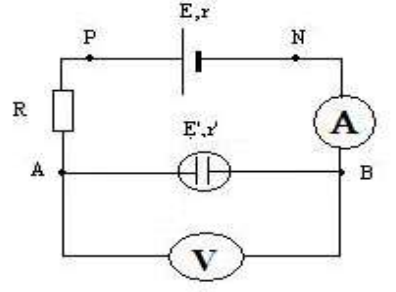
\includegraphics[width=0.15\textwidth]{./img/serie_cercuit.png}
%\end{wrapfigure}
}
    & $1pt$\\\hline
 %Q2
 $2.a$ &
         \makecell{
             L’énergie dissipée par effet joule par le conducteur\\ ohmique : On a : I = 500mA = 0,5 A et $\Delta{t}$ = 12 min = 12 × 60 = 720s\\
$W_R = R.I^2. \Delta{t} = 10 × 0,5^2 × 720 = 1800 J$
 }
    & $1pt$\\\hline
 %Q2.b
 $2.b$ &
         \makecell{
             Il s’agit d’un circuit en série, on peut appliquer \\la loi de
      Pouillet : $I = \frac{E-E'}{R+r+r'}$ donc $r'  = \frac{E-E'}{I} -R -r =5\Omega$
      }
    & $1pt$\\\hline
%Q2 : 
 $3.a$ &
         \makecell{
             L’énergie totale produite par le générateur : \\
             On maintenant I = 0,35 A et $\Delta{t}$ = 20min = 20 × 60 = 1200 s\\
      $W_e = E.I.\Delta{t} $ donc  $We = 12 × 0,35 × 1200 = 5040 J$
 }
    & $1pt$\\\hline
%3.b
 $3.b$ &
         \makecell{
             L’énergie électrique fournie au circuit par le générateur :
\\$W_f = U_{PN}.I.\Delta{t}= E.I.\Delta{t} - r.I^2.\Delta{t}$\\
      donc $W_f = 12 × 0,35 × 1200 - 1 x 0,352 x 1200 = 4893 J$
  }
    & $1pt$\\\hline
%3.c
 $3.c$ &
         \makecell{
             On peut appliquer la loi de Pouillet puisque le\\ circuit est en série : I=$\frac{E-E'}{R + r+ r'}$ alors R = $\frac{E-E'}{I} - r-r' = 17\Omega$
             \\Les dipôles récepteurs qui dissipent de l’énergie\\ par effet joule sont le conducteur ohmique et le
moteur.
\\$W_{th} = R.I^2.\Delta{t} = 3200J$
  }
    & $1pt$\\\hline


      %Partie 2 : -----
\multicolumn{3}{||c||}{\bf{Partie 2 :Bilan énergétique \dotfill (7pts)} }\\
\hline
%1
 $1.$ &
      \makecell{
          $P_r = (R + r')I^2 = 0.32W$
      }
    & $1pt$\\\hline
%2
 $2.$ &
      \makecell{$P_u = E'I = 0.24W$}
    & $1pt$\\\hline
%3
 $3.$ &
      \makecell{$P_e = P_j+ P_u = 0.56W$}
    & $1pt$\\\hline
%4
 $4.a$ &
      \makecell{ $P_j = 0.36-0.32=0.04W$}
    & $1pt$\\\hline
    %4.b
 $4.b$ &
      \makecell{$P_j = rI^2 $ donc $r = \frac{P_J}{I^2} = 4\Omega$}
    & $1pt$\\\hline
    %5
 $5$ &
      \makecell{$P_e = U_{PN}.I= (E-rI)I$ donc $E = \frac{P_e}{I} + rI = 6V$\\
     $I = \frac{E-E'}{R+r+r'} = 0.1A$ } 
    & $2pt$\\\hline



  \end{tabular}
  \end{center}



\end{document}
